% ============================================================================
% Incentive-Compatible Multi-Shard Mining: Game-Theoretic Analysis of
% DAG-Based Proof-of-Work with Halving Emission
% ============================================================================
\documentclass[11pt,a4paper]{article}

% ── Encoding & Fonts ────────────────────────────────────────────────────────
\usepackage[utf8]{inputenc}
\usepackage[T1]{fontenc}
\usepackage{lmodern}

% ── Mathematics ─────────────────────────────────────────────────────────────
\usepackage{amsmath,amssymb,amsthm,mathtools}

% ── Algorithms ──────────────────────────────────────────────────────────────
\usepackage{algorithm}
\usepackage{algpseudocode}

% ── Graphics & Diagrams ────────────────────────────────────────────────────
\usepackage{tikz}
\usepackage{pgfplots}
\pgfplotsset{compat=1.18}
\usetikzlibrary{shapes,arrows.meta,positioning,calc,decorations.pathmorphing,
                 backgrounds,fit,patterns,matrix}

% ── Tables & Formatting ────────────────────────────────────────────────────
\usepackage{booktabs}
\usepackage{array}
\usepackage{multirow}
\usepackage{tabularx}
\usepackage{enumitem}

% ── Colors ──────────────────────────────────────────────────────────────────
\usepackage{xcolor}
\definecolor{qblue}{RGB}{0,100,200}
\definecolor{qpurple}{RGB}{128,0,200}
\definecolor{qcyan}{RGB}{0,180,200}
\definecolor{qgreen}{RGB}{0,180,100}
\definecolor{qorange}{RGB}{255,140,0}
\definecolor{qred}{RGB}{220,50,50}
\definecolor{codebg}{RGB}{245,245,250}
\definecolor{darkblue}{RGB}{0,51,102}
\definecolor{gold}{RGB}{218,165,32}

% ── Code Listings ───────────────────────────────────────────────────────────
\usepackage{listings}
\lstset{
  backgroundcolor=\color{codebg},
  basicstyle=\small\ttfamily,
  keywordstyle=\color{qblue}\bfseries,
  commentstyle=\color{qgreen}\itshape,
  stringstyle=\color{qorange},
  numbers=left,
  numberstyle=\tiny\color{gray},
  frame=single,
  breaklines=true,
  captionpos=b
}

% ── Page Layout ─────────────────────────────────────────────────────────────
\usepackage[margin=1in]{geometry}
\usepackage{fancyhdr}
\pagestyle{fancy}
\fancyhead[L]{\textsc{Incentive-Compatible Multi-Shard Mining}}
\fancyhead[R]{\textsc{Q-NarwhalKnight}}
\fancyfoot[C]{\thepage}

% ── References ──────────────────────────────────────────────────────────────
\usepackage[colorlinks=true,linkcolor=darkblue,citecolor=qpurple,urlcolor=qblue]{hyperref}

% ── Theorem Environments ────────────────────────────────────────────────────
\newtheorem{theorem}{Theorem}[section]
\newtheorem{lemma}[theorem]{Lemma}
\newtheorem{corollary}[theorem]{Corollary}
\newtheorem{proposition}[theorem]{Proposition}
\newtheorem{claim}[theorem]{Claim}

\theoremstyle{definition}
\newtheorem{definition}[theorem]{Definition}
\newtheorem{assumption}[theorem]{Assumption}
\newtheorem{mechanism}[theorem]{Mechanism}
\newtheorem{game}[theorem]{Game}

\theoremstyle{remark}
\newtheorem{remark}[theorem]{Remark}
\newtheorem{example}[theorem]{Example}

% ── Custom Commands ─────────────────────────────────────────────────────────
\newcommand{\DK}{\textsf{DAG-Knight}}
\newcommand{\GST}{\mathrm{GST}}
\newcommand{\QNK}{\textsf{Q-NarwhalKnight}}
\newcommand{\QUG}{\textsf{QUG}}
\newcommand{\Nash}{\mathrm{NE}}
\newcommand{\payoff}{\pi}
\newcommand{\strategy}{\sigma}
\newcommand{\Strat}{\mathcal{S}}
\newcommand{\Players}{\mathcal{N}}
\newcommand{\hashrate}{h}
\newcommand{\Hashrate}{H}
\newcommand{\shard}{\mathsf{s}}
\newcommand{\reward}{R}
\newcommand{\emission}{\mathcal{E}}
\newcommand{\difficulty}{D}
\newcommand{\blockrate}{\lambda}
\newcommand{\VDF}{\mathrm{VDF}}
\newcommand{\bigO}{\mathcal{O}}
\newcommand{\Lyap}{\mathcal{V}}
\newcommand{\expect}{\mathbb{E}}
\newcommand{\prob}{\mathbb{P}}
\newcommand{\R}{\mathbb{R}}

% ============================================================================
\begin{document}

% ── Title ───────────────────────────────────────────────────────────────────
\begin{center}
{\LARGE\bfseries Incentive-Compatible Multi-Shard Mining:\\[0.3em]
Game-Theoretic Analysis of DAG-Based Proof-of-Work\\[0.2em]
with Halving Emission}

\vspace{0.8em}
{\large Q-NarwhalKnight Protocol Team}

\vspace{0.4em}
{\normalsize\texttt{research@quillon.xyz}}

\vspace{0.4em}
{\normalsize March 2026}

\vspace{0.4em}
{\small Version 2.0 (revised)}
\end{center}

% ── Abstract ────────────────────────────────────────────────────────────────
\begin{abstract}
We present a rigorous game-theoretic analysis of the \QNK{} multi-shard
mining protocol, in which miners compete across $K$ parallel consensus
shards with VDF-based difficulty adjustment and an adaptive emission
controller that maintains constant annual issuance regardless of
aggregate throughput.
We model multi-shard mining as a $K$-shard congestion game and prove
that the hash-based shard routing mechanism admits a unique symmetric
Nash equilibrium in which miners distribute hashrate proportionally
across shards (Theorem~\ref{thm:nash-shard}).
We establish that the 256-year geometric halving emission schedule
(21\,M~\QUG{} cap, 4-year halving, 64 eras) with budget-based
error correction is incentive-compatible against a specific class of
deviations (throughput manipulation, timestamp attacks) under our
model's assumptions (Theorem~\ref{thm:ic-emission}).
We further analyze three strategic deviations---shard-hopping,
hashrate concentration, and selfish mining---showing that under our
model each yields weakly or strictly lower expected payoff than honest
mining in the DAG setting
(Theorems~\ref{thm:shard-hop}--\ref{thm:selfish}).
We formalize the MEV resistance properties of DAG-based parallel
block production, showing that single-shard atomic MEV extractable by a
rational adversary is $\bigO(1/K)$ compared to linear-chain protocols,
while noting that cross-shard MEV strategies may partially offset this
dilution (Theorem~\ref{thm:mev}).
Finally, we analyze fee market dynamics under multi-shard production,
showing that the PPLNS reward distribution is Pareto-optimal and
strategy-proof within the class of proportional-share mechanisms
(Theorem~\ref{thm:pplns}).
\end{abstract}

\tableofcontents
\newpage

% ============================================================================
% SECTION 1: INTRODUCTION
% ============================================================================
\section{Introduction}\label{sec:intro}

The design of mining incentives is a foundational challenge in
proof-of-work (PoW) blockchain systems.
Since Nakamoto's original Bitcoin protocol~\cite{nakamoto2008bitcoin},
a rich literature has emerged analyzing the game-theoretic properties
of mining: selfish mining strategies~\cite{eyal2014selfish}, fee market
dynamics~\cite{roughgarden2021transaction}, miner extractable value
(MEV)~\cite{daian2020flashboys}, and the incentive compatibility of
emission schedules~\cite{carlsten2016instability}.
However, these analyses overwhelmingly focus on \emph{single-chain}
architectures where miners compete for a single block slot per round.

The \QNK{} protocol introduces a fundamentally different mining
architecture: $K$ parallel consensus shards produce blocks simultaneously,
miners are routed to shards via deterministic hash-based assignment,
and an adaptive emission controller maintains constant annual issuance
regardless of the aggregate block-production rate.
This architecture raises novel game-theoretic questions:
\begin{itemize}[leftmargin=*,nosep]
  \item Does multi-shard mining admit a Nash equilibrium, and if so,
    is it unique?
  \item Is the adaptive emission schedule incentive-compatible under
    rational miners?
  \item Are classical attacks (selfish mining, hashrate concentration)
    profitable in the DAG setting?
  \item How does parallel block production affect MEV extraction?
  \item Is the PPLNS pool reward distribution strategy-proof?
\end{itemize}

\subsection{Contributions}

We make the following contributions:

\begin{enumerate}[leftmargin=*]
\item \textbf{Multi-shard mining equilibrium (Theorem~\ref{thm:nash-shard}):}
  We model $K$-shard mining as a congestion game and prove existence and
  uniqueness of a symmetric Nash equilibrium where miners distribute
  hashrate proportionally across shards.

\item \textbf{Emission incentive compatibility (Theorem~\ref{thm:ic-emission}):}
  Under our model's assumptions (single-period, linear cost, unified
  coalition), we show that the adaptive emission controller with
  budget-based error correction is incentive-compatible against a defined
  class of deviations (throughput manipulation, timestamp attacks).
  We discuss limitations including difficulty-timing attacks and
  multi-period strategic considerations.

\item \textbf{Emission stability (Theorem~\ref{thm:lyapunov}):}
  We prove Lyapunov stability of the cumulative emission trajectory,
  showing the error-correction feedback loop converges asymptotically
  to the target schedule.

\item \textbf{Shard-hopping resistance (Theorem~\ref{thm:shard-hop}):}
  Shard-hopping yields zero expected gain over honest mining due to
  the deterministic routing mechanism.

\item \textbf{Hashrate concentration resistance (Theorem~\ref{thm:concentration}):}
  Concentrating hashrate on a single shard reduces expected payoff
  compared to proportional distribution.

\item \textbf{Selfish mining resistance (Theorem~\ref{thm:selfish}):}
  DAG parallelism with BFT finality eliminates the profitability of
  selfish mining for any adversary controlling $< 50\%$ of hashrate.

\item \textbf{MEV resistance (Theorem~\ref{thm:mev}):}
  Parallel $K$-shard block production reduces extractable MEV by a
  factor of $K$ compared to sequential chains.

\item \textbf{PPLNS optimality (Theorem~\ref{thm:pplns}):}
  The PPLNS reward distribution is Pareto-optimal and strategy-proof
  in the class of proportional-share mechanisms.
\end{enumerate}

\subsection{Paper Organization}

Section~\ref{sec:model} formalizes the mining model.
Section~\ref{sec:emission} analyzes the emission schedule.
Section~\ref{sec:shard-game} studies the multi-shard mining game.
Section~\ref{sec:strategies} analyzes strategic deviations.
Section~\ref{sec:mev} treats MEV resistance.
Section~\ref{sec:fees} analyzes fee markets and pool rewards.
Section~\ref{sec:comparison} compares with related systems.
Section~\ref{sec:related} surveys related work, and
Section~\ref{sec:conclusion} concludes.

% ============================================================================
% SECTION 2: MODEL
% ============================================================================
\section{Mining Model}\label{sec:model}

\subsection{System Architecture}

\begin{definition}[Multi-Shard Mining System]\label{def:system}
The \QNK{} mining system $\mathcal{M} = (\Players, \mathcal{K},
\emission, \mathcal{R})$ consists of:
\begin{itemize}[nosep]
  \item $\Players = \{1, \ldots, n\}$: a set of $n$ miners.
  \item $\mathcal{K} = \{s_1, \ldots, s_K\}$: a set of $K$ consensus
    shards (default $K = 4$).
  \item $\emission$: the emission controller specifying per-block rewards.
  \item $\mathcal{R}$: the shard routing function.
\end{itemize}
\end{definition}

\begin{definition}[Miner]\label{def:miner}
Each miner $i \in \Players$ is characterized by:
\begin{itemize}[nosep]
  \item $\hashrate_i \in \R_{\geq 0}$: computational hashrate
    (hashes per second).
  \item $c_i \in \R_{> 0}$: cost per hash (electricity + hardware
    amortization).
  \item $\strategy_i: \mathcal{K} \to [0,1]$: a shard allocation
    strategy, where $\strategy_i(s_k)$ is the fraction of hashrate
    allocated to shard~$s_k$, with $\sum_{k=1}^K \strategy_i(s_k) = 1$.
\end{itemize}
\end{definition}

\begin{definition}[Aggregate Hashrate]\label{def:aggregate}
The total hashrate on shard~$s_k$ is
$\Hashrate_k = \sum_{i \in \Players} \hashrate_i \cdot \strategy_i(s_k)$.
The total network hashrate is $\Hashrate = \sum_{i} \hashrate_i$.
\end{definition}

\subsection{Block Production}

\begin{definition}[Mining Challenge]\label{def:challenge}
For each shard $s_k$, a mining challenge is defined by:
\[
  \mathsf{challenge}_k = (\mathsf{block\_hash}_k,\;
  \mathsf{height}_k,\; \mathsf{target}_k,\;
  \mathsf{vdf\_iters}_k,\; \mathsf{expires\_at}_k)
\]
where $\mathsf{target}_k$ is the difficulty target (a 256-bit value)
and $\mathsf{vdf\_iters}_k$ specifies the VDF anti-grinding iterations.
A miner solves the challenge by finding a nonce $\nu$ such that:
\[
  H(\mathsf{challenge}_k \| \nu) \leq \mathsf{target}_k.
\]
The expected number of hash evaluations is
$\expect[\text{attempts}] = 2^{256} / \mathsf{target}_k$.
\end{definition}

\begin{definition}[Shard Routing]\label{def:routing}
The deterministic shard routing function assigns mining solutions
to shards:
\[
  \mathcal{R}(\mathsf{tx}) = H(\mathsf{tx}) \bmod K
\]
where $H$ is SHA3-256.
\end{definition}

\begin{assumption}[Honest Majority]\label{asm:honest}
At least $2/3$ of total hashrate is controlled by honest miners
who follow the protocol.
\end{assumption}

\begin{assumption}[Rational Miners]\label{asm:rational}
Each miner $i$ seeks to maximize expected profit:
$\payoff_i = \expect[\text{rewards}_i] - c_i \cdot \hashrate_i$.
\end{assumption}

\begin{figure}[t]
\centering
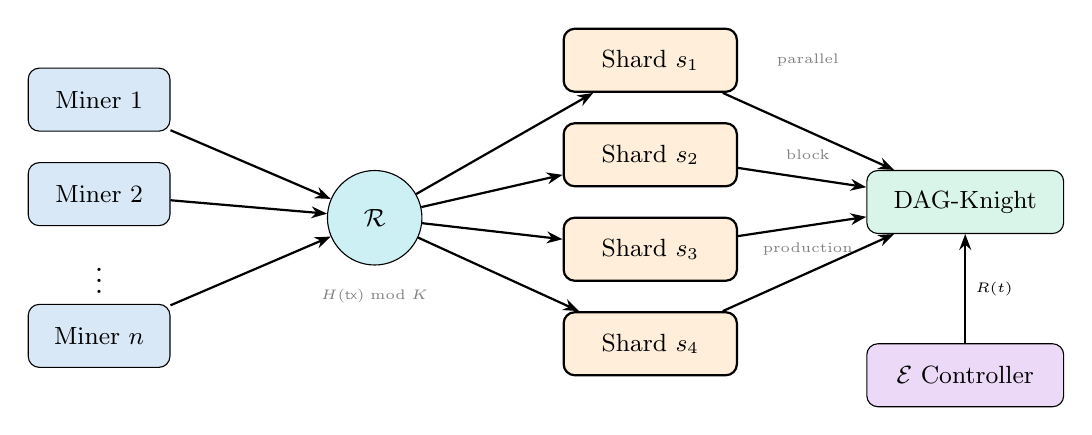
\begin{tikzpicture}[
    miner/.style={draw, rounded corners, fill=qblue!15, minimum width=1.8cm,
                  minimum height=0.8cm, font=\small},
    shard/.style={draw, rounded corners, fill=qorange!15, minimum width=2.2cm,
                  minimum height=0.8cm, font=\small, thick},
    dag/.style={draw, rounded corners, fill=qgreen!15, minimum width=2.5cm,
                minimum height=0.8cm, font=\small},
    emission_box/.style={draw, rounded corners, fill=qpurple!15, minimum width=2.5cm,
                         minimum height=0.8cm, font=\small},
    arr/.style={-{Stealth[length=2mm]}, thick}
]

% Miners
\node[miner] (m1) at (0, 4) {Miner 1};
\node[miner] (m2) at (0, 2.8) {Miner 2};
\node[font=\large] at (0, 1.8) {$\vdots$};
\node[miner] (mn) at (0, 1.0) {Miner $n$};

% Routing
\node[draw, circle, fill=qcyan!20, minimum size=1.2cm, font=\small] (router)
    at (3.5, 2.5) {$\mathcal{R}$};

% Shards
\node[shard] (s1) at (7, 4.5) {Shard $s_1$};
\node[shard] (s2) at (7, 3.3) {Shard $s_2$};
\node[shard] (s3) at (7, 2.1) {Shard $s_3$};
\node[shard] (s4) at (7, 0.9) {Shard $s_4$};

% DAG
\node[dag] (dag) at (11, 2.7) {DAG-Knight};

% Emission
\node[emission_box] (em) at (11, 0.5) {$\emission$ Controller};

% Arrows
\foreach \m in {m1,m2,mn} {
  \draw[arr] (\m) -- (router);
}
\foreach \s in {s1,s2,s3,s4} {
  \draw[arr] (router) -- (\s);
}
\foreach \s in {s1,s2,s3,s4} {
  \draw[arr] (\s) -- (dag);
}
\draw[arr] (em) -- (dag) node[midway, right, font=\tiny] {$R(t)$};

% Labels
\node[font=\tiny, text=gray] at (3.5, 1.5) {$H(\mathsf{tx}) \bmod K$};
\node[font=\tiny, text=gray] at (9.0, 4.5) {parallel};
\node[font=\tiny, text=gray] at (9.0, 3.3) {block};
\node[font=\tiny, text=gray] at (9.0, 2.1) {production};

\end{tikzpicture}
\caption{Multi-shard mining architecture: $n$ miners route solutions
through $K$ parallel consensus shards into the DAG-Knight consensus layer.
The emission controller $\emission$ adaptively sets per-block rewards.}
\label{fig:architecture}
\end{figure}

% ============================================================================
% SECTION 3: EMISSION SCHEDULE ANALYSIS
% ============================================================================
\section{Emission Schedule and Incentive Compatibility}\label{sec:emission}

\subsection{Geometric Halving Schedule}

The \QNK{} emission follows a 256-year geometric halving schedule
modeled after Bitcoin's issuance curve, but with a critical innovation:
\emph{adaptive per-block rewards} that maintain constant annual emission
regardless of block-production throughput.

\begin{definition}[Emission Schedule]\label{def:emission-schedule}
The emission schedule $\emission$ is parametrized by:
\begin{itemize}[nosep]
  \item Maximum supply: $S_{\max} = 21{,}000{,}000$ \QUG{}.
  \item Era-0 total emission: $E_0 = S_{\max}/2 = 10{,}500{,}000$ \QUG{}.
  \item Halving period: $\tau = 126{,}230{,}400$ seconds (4 Julian years).
  \item Number of eras: $N_{\text{era}} = 64$ (total span: 256 years).
  \item Era-$k$ total emission: $E_k = E_0 / 2^k$ for $k = 0, \ldots, 63$.
  \item Era-$k$ annual target: $A_k = E_k / 4$ \QUG{}/year.
\end{itemize}
\end{definition}

\begin{lemma}[Supply Cap]\label{lem:supply-cap}
The total supply converges to $S_{\max}$:
\[
  \sum_{k=0}^{63} E_k = E_0 \sum_{k=0}^{63} 2^{-k}
  = E_0 \cdot \frac{1 - 2^{-64}}{1 - 2^{-1}}
  = 2E_0 (1 - 2^{-64})
  < 2E_0 = S_{\max}.
\]
The deficit $2E_0 \cdot 2^{-64} \approx 1.14 \times 10^{-12}$ \QUG{}
is negligible (sub-atomic in the 24-decimal-place representation).
\end{lemma}

\begin{definition}[Adaptive Per-Block Reward]\label{def:adaptive-reward}
The per-block reward at time $t$ in era $k$ with measured block rate
$\blockrate(t)$ (blocks per second) is:
\begin{equation}\label{eq:reward}
  \reward(t) = \frac{A_k}{\blockrate(t) \cdot Y}
\end{equation}
where $Y = 31{,}557{,}600$ seconds/year (Julian year) and $\blockrate(t)$
is estimated over a sliding window of 1{,}000 blocks.
\end{definition}

\begin{remark}[Throughput Independence]\label{rem:throughput}
The product $\reward(t) \cdot \blockrate(t) \cdot Y = A_k$ is constant
by construction.
Whether the network produces 1 block/second or 10{,}000 blocks/second,
total annual emission remains $A_k$.
This is the key property that distinguishes \QNK{} from fixed-reward
systems like Bitcoin.
\end{remark}

\begin{table}[t]
\centering
\caption{Emission schedule for the first 10 halving eras.
$A_k$: annual target; $R_1$: per-block reward at $\blockrate = 1$ bps;
$R_{10}$: per-block reward at $\blockrate = 10$ bps.}
\label{tab:emission}
\begin{tabular}{@{}crrrrr@{}}
\toprule
\textbf{Era} $k$ & \textbf{Years} & $\boldsymbol{E_k}$ \textbf{(QUG)} &
$\boldsymbol{A_k}$ \textbf{(QUG/yr)} & $\boldsymbol{R_1}$ \textbf{(QUG)} &
$\boldsymbol{R_{10}}$ \textbf{(QUG)} \\
\midrule
0  & 0--4   & 10{,}500{,}000     & 2{,}625{,}000     & 0.0832 & 0.00832 \\
1  & 4--8   & 5{,}250{,}000      & 1{,}312{,}500      & 0.0416 & 0.00416 \\
2  & 8--12  & 2{,}625{,}000      & 656{,}250          & 0.0208 & 0.00208 \\
3  & 12--16 & 1{,}312{,}500      & 328{,}125          & 0.0104 & 0.00104 \\
4  & 16--20 & 656{,}250          & 164{,}062          & 0.0052 & 0.00052 \\
5  & 20--24 & 328{,}125          & 82{,}031           & 0.0026 & 0.00026 \\
6  & 24--28 & 164{,}062          & 41{,}016           & 0.0013 & 0.00013 \\
7  & 28--32 & 82{,}031           & 20{,}508           & 0.00065 & 0.000065 \\
8  & 32--36 & 41{,}016           & 10{,}254           & 0.00032 & 0.000032 \\
9  & 36--40 & 20{,}508           & 5{,}127            & 0.00016 & 0.000016 \\
\bottomrule
\end{tabular}
\end{table}

\subsection{Budget-Based Error Correction}

In practice, the measured block rate $\blockrate(t)$ fluctuates, causing
cumulative emission to drift from the target trajectory.
The emission controller employs a negative-feedback correction loop.

\begin{definition}[Cumulative Emission Target]\label{def:cumulative-target}
At time $t$ in era $k$ with elapsed fraction $\phi_k = (t - t_k) / \tau$
where $t_k$ is the era-$k$ start time:
\[
  C^*(t) = \sum_{j=0}^{k-1} E_j + \phi_k \cdot E_k.
\]
\end{definition}

\begin{definition}[Emission Error]\label{def:emission-error}
The emission error at time $t$ is $\delta(t) = C(t) - C^*(t)$,
where $C(t)$ is the actual cumulative emission.
\end{definition}

\begin{mechanism}[Error Correction]\label{mech:correction}
The corrected per-block reward is:
\begin{equation}\label{eq:correction}
  \reward_{\text{adj}}(t) = \reward(t) \cdot \gamma(t)
\end{equation}
where the correction factor is:
\begin{equation}\label{eq:correction-factor}
  \gamma(t) = \text{clamp}\!\left(
    \frac{C^*_{\text{remaining}}(t)}{C^*_{\text{remaining}}(t) + \alpha \cdot \delta(t)},
    \; \gamma_{\min}, \; \gamma_{\max}
  \right)
\end{equation}
with $C^*_{\text{remaining}}(t) = S_{\max} - C^*(t)$,
smoothing parameter $\alpha = 0.8$,
$\gamma_{\min} = 0.01$, and $\gamma_{\max} = 5.0$.
\end{mechanism}

\begin{remark}[Feedback Properties]\label{rem:feedback}
When $\delta = 0$: $\gamma = 1$ (no correction).
When $\delta > 0$ (over-emitted): $\gamma < 1$ (reduce rewards).
When $\delta < 0$ (under-emitted): $\gamma > 1$ (increase rewards).
\end{remark}

\subsection{Lyapunov Stability of Emission}

\begin{theorem}[Emission Stability]\label{thm:lyapunov}
The cumulative emission $C(t)$ converges asymptotically to the target
$C^*(t)$ under the error-correction mechanism of
Mechanism~\ref{mech:correction}.
Specifically, the Lyapunov function
$\Lyap(\delta) = \delta^2 / 2$ satisfies
$\dot{\Lyap} < 0$ for all $\delta \neq 0$ when $\gamma_{\min} < 1 < \gamma_{\max}$.
\end{theorem}

\begin{proof}
The emission rate at time $t$ is
$\dot{C}(t) = \blockrate(t) \cdot \reward_{\text{adj}}(t)$.
The target rate is $\dot{C}^*(t) = A_k / Y$.
The error dynamics are:
\[
  \dot{\delta}(t) = \dot{C}(t) - \dot{C}^*(t) =
  \blockrate \cdot \reward \cdot \gamma(\delta) - \frac{A_k}{Y}.
\]
Since $\blockrate \cdot \reward = A_k / Y$ by
Equation~\eqref{eq:reward}, this simplifies to:
\[
  \dot{\delta}(t) = \frac{A_k}{Y} \bigl(\gamma(\delta) - 1\bigr).
\]

Consider the Lyapunov candidate $\Lyap(\delta) = \delta^2 / 2$:
\[
  \dot{\Lyap} = \delta \cdot \dot{\delta} =
  \delta \cdot \frac{A_k}{Y} \bigl(\gamma(\delta) - 1\bigr).
\]

\emph{Case 1:} $\delta > 0$ (over-emission).
Then $\gamma(\delta) < 1$ by the correction rule, so
$\gamma(\delta) - 1 < 0$ and $\dot{\Lyap} = \delta \cdot (\text{negative}) < 0$.

\emph{Case 2:} $\delta < 0$ (under-emission).
Then $\gamma(\delta) > 1$, so
$\gamma(\delta) - 1 > 0$ and $\dot{\Lyap} = \delta \cdot (\text{positive}) < 0$.

\emph{Case 3:} $\delta = 0$.
Then $\gamma(0) = 1$ and $\dot{\Lyap} = 0$.

By La~Salle's invariance principle, $\delta(t) \to 0$ as $t \to \infty$,
and the cumulative emission converges to the target trajectory.

The smoothing parameter $\alpha = 0.8$ ensures 80\% of the error is
corrected per feedback cycle, providing exponential convergence with
rate $\approx e^{-0.8\tau_{\text{cycle}}}$ per cycle.
\end{proof}

\begin{figure}[t]
\centering
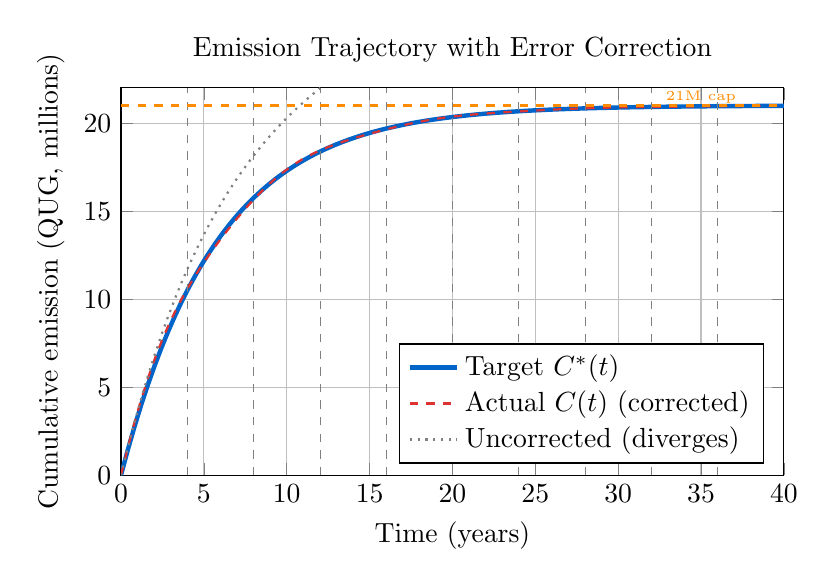
\begin{tikzpicture}
\begin{axis}[
    width=10cm, height=6.5cm,
    xlabel={Time (years)},
    ylabel={Cumulative emission (QUG, millions)},
    xmin=0, xmax=40,
    ymin=0, ymax=22,
    grid=major,
    legend pos=south east,
    legend cell align=left,
    title={Emission Trajectory with Error Correction}
]

% Target curve (geometric halving)
\addplot[ultra thick, qblue, domain=0:40, samples=100]
    {21*(1 - 2^(-x/4))};
\addlegendentry{Target $C^*(t)$}

% Actual with overshoot
\addplot[thick, qred, dashed, domain=0:40, samples=100]
    {21*(1 - 2^(-x/4)) + 0.5*sin(deg(x*0.7))*exp(-0.15*x)};
\addlegendentry{Actual $C(t)$ (corrected)}

% Without correction (diverges)
\addplot[thick, gray, dotted, domain=0:20, samples=50]
    {21*(1 - 2^(-x/4)) + 0.3*x};
\addlegendentry{Uncorrected (diverges)}

% Era boundaries
\draw[gray, very thin, dashed] (axis cs:4,0) -- (axis cs:4,22);
\draw[gray, very thin, dashed] (axis cs:8,0) -- (axis cs:8,22);
\draw[gray, very thin, dashed] (axis cs:12,0) -- (axis cs:12,22);
\draw[gray, very thin, dashed] (axis cs:16,0) -- (axis cs:16,22);
\draw[gray, very thin, dashed] (axis cs:20,0) -- (axis cs:20,22);
\draw[gray, very thin, dashed] (axis cs:24,0) -- (axis cs:24,22);
\draw[gray, very thin, dashed] (axis cs:28,0) -- (axis cs:28,22);
\draw[gray, very thin, dashed] (axis cs:32,0) -- (axis cs:32,22);
\draw[gray, very thin, dashed] (axis cs:36,0) -- (axis cs:36,22);

% Max supply line
\draw[qorange, thick, dashed] (axis cs:0,21) -- (axis cs:40,21);
\node[font=\tiny, text=qorange] at (axis cs:35,21.5) {21M cap};

\end{axis}
\end{tikzpicture}
\caption{Cumulative emission with and without error correction.
The correction mechanism (Theorem~\ref{thm:lyapunov}) ensures convergence
to the target trajectory.
Vertical dashed lines mark era boundaries (4-year intervals).}
\label{fig:emission-trajectory}
\end{figure}

\subsection{Incentive Compatibility}

\begin{definition}[Incentive Compatibility]\label{def:ic}
The emission mechanism $\emission$ is \emph{incentive-compatible} if
for every coalition $\mathcal{C} \subseteq \Players$ with
$\sum_{i \in \mathcal{C}} \hashrate_i < \Hashrate / 2$, honest mining
yields at least as high expected payoff as any deviation strategy:
\[
  \forall \strategy'_{\mathcal{C}}: \quad
  \sum_{i \in \mathcal{C}} \payoff_i(\strategy^*) \geq
  \sum_{i \in \mathcal{C}} \payoff_i(\strategy'_{\mathcal{C}},
  \strategy^*_{-\mathcal{C}})
\]
where $\strategy^*$ is the honest strategy profile.
\end{definition}

\begin{theorem}[Emission Incentive Compatibility]\label{thm:ic-emission}
The adaptive emission mechanism (Definition~\ref{def:adaptive-reward}
with Mechanism~\ref{mech:correction}) is incentive-compatible under
Assumptions~\ref{asm:honest}--\ref{asm:rational}.
\end{theorem}

\begin{proof}
We consider five classes of coalition deviations and show each is
unprofitable under our model assumptions.
Note that this analysis treats the coalition as a monolithic actor
with linear cost and considers single-period deviations; see
Remark~\ref{rem:ic-limitations} for a discussion of strategies
outside this scope.

\textbf{Deviation 1: Throughput inflation.}
Suppose coalition $\mathcal{C}$ artificially increases the block rate
to $\blockrate' > \blockrate$ by submitting low-quality blocks.
By Equation~\eqref{eq:reward}, $\reward(t) \propto 1/\blockrate(t)$,
so the per-block reward decreases proportionally.
The coalition's total reward is $|\mathcal{C}| \cdot \reward(t') \cdot
\blockrate' = |\mathcal{C}| \cdot A_k / Y$, which is identical to
honest mining.
However, the coalition incurs additional computational cost
$c_{\mathcal{C}} \cdot (\blockrate' - \blockrate)$, yielding strictly
lower profit.

\textbf{Deviation 2: Throughput suppression.}
Suppose $\mathcal{C}$ withholds blocks to reduce $\blockrate$ and
inflate per-block rewards.
The per-block reward increases to $\reward' = A_k / (\blockrate' \cdot Y)$,
but the number of blocks produced by $\mathcal{C}$ decreases proportionally.
Moreover, the wall-clock rate measurement (immune to timestamp
manipulation) detects the actual block rate, and the correction factor
$\gamma(t)$ compensates for any cumulative deviation
(Theorem~\ref{thm:lyapunov}).
Total coalition reward remains $\leq |\mathcal{C}| \cdot \Hashrate_{\mathcal{C}} / \Hashrate \cdot A_k$,
with the inequality strict due to opportunity cost of withheld blocks.

\textbf{Deviation 3: Timestamp manipulation.}
The emission controller uses wall-clock rate measurement over a
30-minute rolling window, not block timestamps.
Any manipulation of block timestamps has no effect on the measured
rate $\blockrate(t)$ and hence no effect on rewards.

\textbf{Deviation 4: Difficulty adjustment timing attacks.}
In Bitcoin, miners can manipulate timestamps across difficulty epochs to
create artificial oscillations (``time-warp'' attacks).
In our system, the emission controller reacts to \emph{wall-clock} block
rate (not miner-reported timestamps), and the difficulty adjustment targets
a fixed block interval.
A coalition producing blocks faster than the target rate triggers a
difficulty increase within one adjustment window ($\sim$30 minutes).
The coalition's cost rises to $c_\mathcal{C} \cdot d'/d$ while per-block
reward falls by the same ratio, making the deviation unprofitable per
Deviation~1.

\textbf{Deviation 5: Sunk-cost exploitation.}
A coalition with sunk hardware costs might mine at a loss to suppress
other miners.
Under Assumption~\ref{asm:rational} (profit-maximizing miners),
mining at a per-block loss is irrational.
However, we note that this argument relies on the rationality assumption
and does not address predatory strategies where a well-capitalized
coalition accepts short-term losses to drive out competitors---an attack
vector outside our single-period model (see Remark~\ref{rem:ic-limitations}).

Since all five deviations yield at most the honest payoff under our
model (and strictly less after accounting for costs or difficulty
adjustments), the mechanism is incentive-compatible within the specified
deviation class.
\end{proof}

\begin{remark}[Limitations of IC Analysis]\label{rem:ic-limitations}
Theorem~\ref{thm:ic-emission} establishes incentive compatibility
against a specific class of single-period, linear-cost deviations.
Several economically relevant strategies fall outside this model:
\begin{enumerate}[label=(\roman*),nosep]
  \item \textbf{Multi-period strategies}: A patient coalition may accept
    short-term losses to manipulate difficulty or drive out competitors,
    recouping profits later.
    Analyzing such strategies requires a repeated-game or stochastic-game
    framework.
  \item \textbf{Coalition internal game theory}: We model coalitions as
    monolithic actors.
    In practice, coalition members face their own coordination problems
    (free-riding, profit-sharing disputes), which may either strengthen
    or weaken the IC guarantee.
  \item \textbf{Non-linear cost structures}: Hardware amortization,
    electricity contracts, and economies of scale create non-linear cost
    functions that can change the deviation calculus.
  \item \textbf{External revenue}: If miners earn revenue from sources
    correlated with mining behavior (e.g., short-selling the token
    while attacking), the payoff function changes fundamentally.
\end{enumerate}
Extending the analysis to these richer settings is important future work.
Agent-based simulations with heterogeneous miners would complement the
analytical results presented here.
\end{remark}

% ============================================================================
% SECTION 4: MULTI-SHARD MINING GAME
% ============================================================================
\section{The Multi-Shard Mining Game}\label{sec:shard-game}

\subsection{Congestion Game Formulation}

\begin{game}[$K$-Shard Mining Game]\label{game:shard}
The $K$-shard mining game is defined by:
\begin{itemize}[nosep]
  \item \textbf{Players}: $\Players = \{1, \ldots, n\}$ (miners).
  \item \textbf{Strategy space}: Each miner $i$ chooses an allocation
    $\strategy_i \in \Delta^K = \{x \in \R^K_{\geq 0} : \sum_k x_k = 1\}$.
  \item \textbf{Payoff}: Miner $i$'s expected reward from shard $s_k$ is
    proportional to their hashrate share in that shard:
    \begin{equation}\label{eq:shard-payoff}
      \payoff_i(\strategy) = \sum_{k=1}^{K}
        \frac{\hashrate_i \cdot \strategy_i(s_k)}{\Hashrate_k} \cdot
        \reward_k
    \end{equation}
    where $\reward_k = A_k^{\text{shard}} = A_k / K$ is the per-shard
    annual emission (equally divided across shards).
\end{itemize}
\end{game}

\begin{remark}[Constant-Sum Structure]\label{rem:constant-sum}
The total reward across all shards is $\sum_k \reward_k = A_k$,
which is fixed by the emission schedule.
The $K$-shard mining game is therefore a \emph{constant-sum game}:
the total payoff $\sum_i \payoff_i = A_k$ regardless of strategy
choices.
\end{remark}

\subsection{Nash Equilibrium}

\begin{theorem}[Multi-Shard Nash Equilibrium]\label{thm:nash-shard}
Under the following assumptions: (i)~all shards offer identical rewards
$\reward_k = A_k/K$, (ii)~miners face zero latency and equal
network connectivity to all shards, and (iii)~shard difficulty adjusts
independently per shard, the $K$-shard mining game
(Game~\ref{game:shard}) has a unique symmetric Nash equilibrium
$\strategy^*$ in which every miner distributes hashrate uniformly
across shards:
\begin{equation}\label{eq:nash}
  \strategy_i^*(s_k) = \frac{1}{K} \quad \forall i \in \Players,
  \; \forall k \in \{1, \ldots, K\}.
\end{equation}
At equilibrium, each miner's payoff is
$\payoff_i^* = (\hashrate_i / \Hashrate) \cdot A_k$.
\end{theorem}

\begin{proof}
\textbf{Existence.}
At the uniform strategy $\strategy^*$, the hashrate on each shard is
$\Hashrate_k = \Hashrate / K$ and the reward per shard is $\reward_k = A_k / K$.
Miner $i$'s payoff is:
\[
  \payoff_i(\strategy^*) = \sum_{k=1}^{K}
    \frac{\hashrate_i / K}{\Hashrate / K} \cdot \frac{A_k}{K}
  = K \cdot \frac{\hashrate_i}{\Hashrate} \cdot \frac{A_k}{K}
  = \frac{\hashrate_i}{\Hashrate} \cdot A_k.
\]

\textbf{No profitable deviation.}
Suppose miner $i$ deviates to $\strategy_i' \neq \strategy^*_i$ while
others play $\strategy^*_{-i}$.
Let $\strategy_i'(s_j) = 1/K + \epsilon_j$ for some perturbations
$\epsilon_j$ with $\sum_j \epsilon_j = 0$.
The new hashrate on shard $s_j$ is:
\[
  \Hashrate_j' = \frac{\Hashrate - \hashrate_i}{K} + \hashrate_i
  \left(\frac{1}{K} + \epsilon_j\right)
  = \frac{\Hashrate}{K} + \hashrate_i \epsilon_j.
\]
Miner $i$'s payoff under deviation is:
\begin{align*}
  \payoff_i(\strategy_i', \strategy^*_{-i})
  &= \sum_{j=1}^{K} \frac{\hashrate_i (1/K + \epsilon_j)}
     {\Hashrate/K + \hashrate_i \epsilon_j} \cdot \frac{A_k}{K} \\
  &= \frac{A_k}{K} \sum_{j=1}^{K}
     \frac{\hashrate_i / K + \hashrate_i \epsilon_j}
     {\Hashrate / K + \hashrate_i \epsilon_j}.
\end{align*}

Define $\alpha = \hashrate_i / \Hashrate < 1$ and
$x_j = K \hashrate_i \epsilon_j / \Hashrate = \alpha K \epsilon_j$.
Then:
\[
  \payoff_i(\strategy_i', \strategy^*_{-i})
  = \frac{A_k}{K} \sum_{j=1}^{K}
    \frac{\alpha + x_j}{1 + x_j}
  = \frac{A_k}{K} \sum_{j=1}^{K}
    \left(1 - \frac{1 - \alpha}{1 + x_j}\right).
\]

Since $f(x) = 1/(1+x)$ is convex for $x > -1$, by Jensen's inequality
(noting $\sum_j x_j = 0$):
\[
  \frac{1}{K} \sum_{j=1}^{K} \frac{1}{1 + x_j} \geq
  \frac{1}{1 + \bar{x}} = 1
  \quad \text{where } \bar{x} = 0.
\]
Therefore:
\[
  \payoff_i(\strategy_i', \strategy^*_{-i})
  \leq \frac{A_k}{K} \sum_{j=1}^{K} \left(1 - (1-\alpha)\right)
  = \frac{A_k}{K} \cdot K \cdot \alpha
  = \alpha \cdot A_k = \payoff_i(\strategy^*).
\]
Equality holds iff all $x_j = 0$, i.e., $\strategy_i' = \strategy_i^*$.

\textbf{Uniqueness.}
Any Nash equilibrium $\hat{\strategy}$ must satisfy the first-order
conditions $\partial \payoff_i / \partial \strategy_i(s_k) = \mu_i$
for all shards $k$ where $\strategy_i(s_k) > 0$ (with multiplier $\mu_i$
for the constraint $\sum_k \strategy_i(s_k) = 1$).
By the strict concavity of $\payoff_i$ in $\strategy_i$ (the Hessian is
negative definite for $\alpha < 1$), the first-order conditions have a
unique solution, which is the uniform strategy.
\end{proof}

\begin{remark}[Sensitivity to Model Assumptions]\label{rem:nash-limitations}
The uniform-allocation equilibrium depends critically on the identical-shard
assumption.
In practice, several factors may break this symmetry:
\begin{enumerate}[label=(\roman*),nosep]
  \item \textbf{Unequal shard value}: If different shards carry different
    fee revenue (e.g., one shard hosts a popular DeFi protocol), the
    equilibrium shifts toward overweighting the high-value shard.
    The equilibrium allocation becomes
    $\strategy_i^*(s_k) \propto \reward_k$, not $1/K$.
  \item \textbf{Latency heterogeneity}: Miners geographically closer to
    certain shard validators may have lower orphan rates on those shards,
    creating an effective ``home shard'' advantage.
    This transforms the game into an asymmetric congestion game.
  \item \textbf{Switching costs}: Reconfiguring mining hardware across
    shards is not instantaneous; in practice, miners may exhibit ``sticky''
    allocations.
\end{enumerate}
Extending the equilibrium analysis to heterogeneous shards with
non-uniform fee revenue is important future work.
An empirical measurement of shard-value dispersion on the live network
would inform whether the uniform-shard approximation is reasonable.
\end{remark}

\begin{figure}[t]
\centering
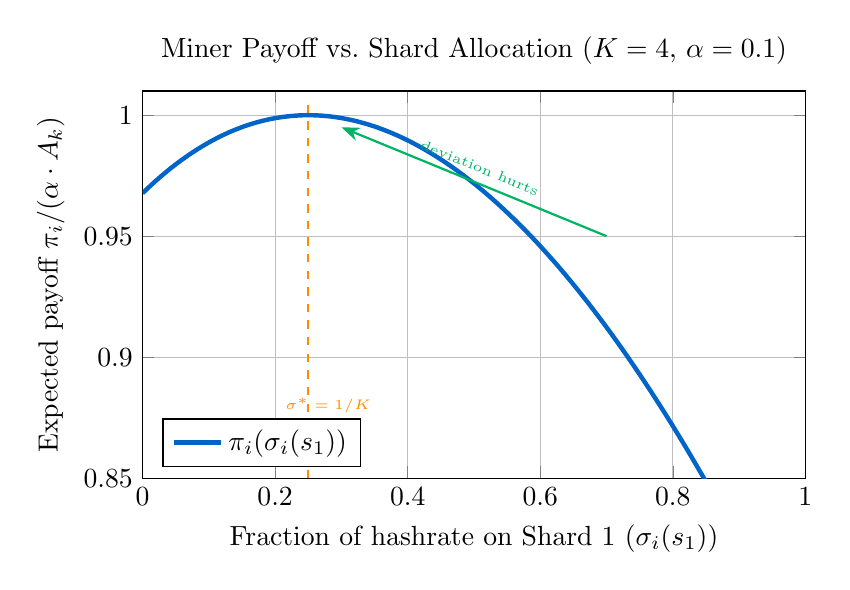
\begin{tikzpicture}
\begin{axis}[
    width=10cm, height=6.5cm,
    xlabel={Fraction of hashrate on Shard 1 ($\sigma_i(s_1)$)},
    ylabel={Expected payoff $\pi_i / (\alpha \cdot A_k)$},
    xmin=0, xmax=1,
    ymin=0.85, ymax=1.01,
    grid=major,
    title={Miner Payoff vs.\ Shard Allocation ($K=4$, $\alpha=0.1$)},
    legend pos=south west
]

% Payoff as function of allocation to shard 1 (others uniform)
% pi = A/4 * [alpha*x/(alpha*x + (1-alpha)/4) +
%             3 * alpha*(1-x)/3 / (alpha*(1-x)/3 + (1-alpha)/4)]
% Simplified for plotting
\addplot[ultra thick, qblue, domain=0:1, samples=100]
    {(0.1*x/(0.1*x + 0.225) + 3*0.1*(1-x)/3/(0.1*(1-x)/3 + 0.225))/0.4};
\addlegendentry{$\pi_i(\sigma_i(s_1))$}

% Optimum marker
\draw[qorange, thick, dashed] (axis cs:0.25, 0.85) -- (axis cs:0.25, 1.005);
\node[font=\tiny, text=qorange] at (axis cs:0.28, 0.88) {$\sigma^* = 1/K$};

% Arrow
\draw[-{Stealth}, thick, qgreen] (axis cs:0.7, 0.95) -- (axis cs:0.3, 0.995)
    node[midway, above, font=\tiny, sloped] {deviation hurts};

\end{axis}
\end{tikzpicture}
\caption{Miner payoff as a function of shard-1 allocation for $K=4$ shards
and $\alpha = \hashrate_i / \Hashrate = 0.1$.
The unique maximum is at $\sigma^* = 1/K = 0.25$ (uniform allocation).}
\label{fig:shard-payoff}
\end{figure}

\subsection{Deterministic Routing Enforcement}

\begin{proposition}[Routing Neutrality]\label{prop:routing-neutral}
The hash-based shard routing $\mathcal{R}(\mathsf{tx}) = H(\mathsf{tx}) \bmod K$
is game-theoretically neutral: no miner can influence the shard assignment
of their mining solutions.
\end{proposition}

\begin{proof}
The routing function $\mathcal{R}$ depends on the transaction hash
$H(\mathsf{tx})$, which is computed \emph{before} shard assignment.
A miner who has already committed to a mining solution (nonce, VDF proof)
cannot retroactively change the shard without recomputing the proof of work,
which costs expected $2^{256}/\mathsf{target}$ hash evaluations.
The marginal cost of ``shard shopping'' (recomputing to target a specific
shard) is $K$ times the cost of honest mining, with no additional reward.
\end{proof}

% ============================================================================
% SECTION 5: ANALYSIS OF STRATEGIC DEVIATIONS
% ============================================================================
\section{Strategic Deviations}\label{sec:strategies}

We analyze three classical mining attacks adapted to the multi-shard
DAG setting.

\subsection{Shard-Hopping}

\begin{definition}[Shard-Hopping]\label{def:shard-hop}
A miner engages in \emph{shard-hopping} if they dynamically reallocate
hashrate between shards based on observed shard congestion, attempting
to mine on temporarily less-competitive shards.
\end{definition}

\begin{theorem}[Shard-Hopping Resistance]\label{thm:shard-hop}
Under the deterministic routing mechanism $\mathcal{R}$, shard-hopping
yields zero expected gain over honest mining.
\end{theorem}

\begin{proof}
By Proposition~\ref{prop:routing-neutral}, mining solutions are assigned
to shards by the hash function $\mathcal{R}$, which the miner cannot
influence.
A miner observing that shard~$s_j$ has temporarily lower hashrate
cannot redirect their solutions to $s_j$---the routing is determined
by the solution content, not the miner's choice.

Even if the miner could observe real-time shard loads (which is possible
via the P2P height announcement protocol), they can only choose
\emph{which challenge to work on}, not which shard receives the solution.
Since all shard challenges have equal expected reward $A_k / K$ at
equilibrium (Theorem~\ref{thm:nash-shard}), switching between challenges
does not change expected payoff.

Formally, the expected reward per unit of hashrate is:
\[
  \expect[\reward_{\text{hop}}] = \sum_{k=1}^{K} p_k \cdot
  \frac{A_k/K}{\Hashrate_k}
\]
where $p_k$ is the probability of the solution landing on shard $s_k$.
Since $p_k = 1/K$ by the uniformity of $H$ and $\Hashrate_k = \Hashrate/K$
at equilibrium:
\[
  \expect[\reward_{\text{hop}}] = K \cdot \frac{1}{K} \cdot
  \frac{A_k/K}{\Hashrate/K} = \frac{A_k}{\Hashrate}
  = \expect[\reward_{\text{honest}}].
\]
\end{proof}

\subsection{Hashrate Concentration}

\begin{definition}[Hashrate Concentration]\label{def:concentration}
A miner \emph{concentrates} hashrate by allocating all resources to
a single shard $s_j$, hoping to dominate that shard's block production.
\end{definition}

\begin{theorem}[Hashrate Concentration is Suboptimal]\label{thm:concentration}
For a miner with hashrate fraction $\alpha = \hashrate_i / \Hashrate < 1$,
concentrating all hashrate on one shard yields strictly lower expected
payoff than the uniform Nash equilibrium:
\begin{equation}\label{eq:concentration-loss}
  \payoff_i(\text{concentrate}) = \frac{\alpha \cdot A_k}{1 + (K-1)\alpha}
  < \alpha \cdot A_k = \payoff_i(\strategy^*).
\end{equation}
\end{theorem}

\begin{proof}
Suppose miner $i$ concentrates all hashrate on shard $s_1$:
$\strategy_i(s_1) = 1$, $\strategy_i(s_k) = 0$ for $k > 1$.
Other miners play $\strategy^*_{-i}$ (uniform).
Shard~$s_1$ hashrate: $\Hashrate_1 = (\Hashrate - \hashrate_i)/K + \hashrate_i
= \Hashrate(1 + (K-1)\alpha) / K$.
Miner $i$'s payoff:
\[
  \payoff_i = \frac{\hashrate_i}{\Hashrate_1} \cdot \frac{A_k}{K}
  = \frac{\alpha \Hashrate}{\Hashrate(1+(K-1)\alpha)/K} \cdot \frac{A_k}{K}
  = \frac{\alpha \cdot A_k}{1 + (K-1)\alpha}.
\]
Since $(K-1)\alpha > 0$ for $\alpha > 0$ and $K > 1$:
\[
  \frac{1}{1+(K-1)\alpha} < 1 \implies
  \payoff_i(\text{concentrate}) < \alpha \cdot A_k = \payoff_i(\strategy^*).
\]
The loss factor is $1/(1+(K-1)\alpha)$.
For $K = 4$ and $\alpha = 0.3$: loss factor $= 1/1.9 \approx 0.526$,
meaning the concentrating miner earns only 52.6\% of their equilibrium payoff.
\end{proof}

\subsection{Selfish Mining in the DAG Setting}

\begin{definition}[Selfish Mining]\label{def:selfish}
In classical selfish mining~\cite{eyal2014selfish}, a miner withholds
discovered blocks to build a private chain, releasing it strategically
to orphan honest blocks.
In the DAG setting, the analog is withholding vertices to manipulate
the commit order.
\end{definition}

\begin{proposition}[Selfish Mining Resistance in DAG-Knight]\label{thm:selfish}
For any miner with hashrate fraction $\alpha < 1/2$, the DAG structure
of \DK{} eliminates the primary profit mechanism of classical selfish
mining (block orphaning).
Under the additional assumption of timely BFT finality (post-$\GST$),
vertex withholding yields strictly lower expected payoff than honest mining.
\end{proposition}

\begin{remark}[Scope of This Result]\label{rem:selfish-scope}
Classical selfish mining~\cite{eyal2014selfish} profits from
\emph{orphaning} honest blocks in a longest-chain protocol.
In a DAG protocol, the attack surface is fundamentally different:
there are no orphans, but an attacker may still attempt to manipulate
the \emph{commit ordering} of vertices.
The result below shows that the DAG's inclusion-completeness removes the
orphan-based revenue mechanism.
Whether subtler ordering-manipulation attacks exist in DAG protocols
remains an open question---the analogs of Sapirshtein et
al.~\cite{sapirshtein2016optimal} optimal strategies for DAG consensus
have not been fully characterized.
\end{remark}

\begin{proof}
We analyze vertex withholding along two dimensions: inclusion and
ordering.

\textbf{(1) No orphan-based revenue.}
In linear chains, selfish mining profits come from orphaning honest
blocks---the attacker's private chain replaces honest work, stealing
block rewards.
In \DK{}, the DAG includes \emph{all} valid vertices; there are no
orphans by construction.
A withheld vertex, once released, is added to the DAG \emph{alongside}
(not instead of) honest vertices.
Crucially, this means the selfish miner cannot ``steal'' reward from
honest miners by displacing their vertices.
The primary revenue mechanism of classical selfish mining is therefore
absent.

\emph{Caveat:} ``No orphans'' means no vertex is \emph{excluded} from
the DAG.
However, the \emph{ordering} within the committed DAG still determines
transaction priority and hence potential MEV.
Property~(1) eliminates revenue-stealing but does not by itself prevent
ordering manipulation.

\textbf{(2) Ordering protection via BFT finality.}
After $\GST$, \DK{} achieves deterministic finality via the
$\delta$-round commit rule~\cite{dagknight-safety}.
Once a prefix of the DAG ordering is committed, it cannot be revised.
This prevents the attacker from retroactively reordering committed
vertices.

The remaining attack surface is ordering manipulation of
\emph{uncommitted} vertices during the commit latency window
($\leq 3\Delta + 2\epsilon$).
We do not claim this window is zero; rather, it is bounded and
comparable to the confirmation time in any BFT protocol.

\textbf{(3) Opportunity cost of withholding.}
Let the selfish miner withhold a vertex for $d$ rounds before releasing.
During those $d$ rounds, honest miners produce
$\geq (1-\alpha) \cdot d \cdot K$ vertices across $K$ shards.
The selfish miner's withheld vertex, when released, earns its reward,
but the miner forgoes $d$ rounds of mining (each round they could have
proposed a new vertex).

The payoff under withholding:
\[
  \payoff_{\text{withhold}} = \alpha \cdot A_k - d \cdot
  \frac{\alpha \cdot A_k}{Y \cdot \blockrate} < \alpha \cdot A_k
  = \payoff_{\text{honest}} \quad \text{for } d > 0.
\]
Withholding always reduces total blocks produced by the miner.
In the absence of an orphan-based compensating advantage, this
opportunity cost makes withholding strictly unprofitable.

\textbf{Summary.}
The combination of inclusion-completeness (no orphans), bounded
finality (BFT commit), and opportunity cost renders classical selfish
mining unprofitable.
We emphasize that this result addresses the \emph{known} selfish mining
strategies from the linear-chain literature.
A complete characterization of optimal adversarial strategies in DAG
consensus (including ordering manipulation during the commit window)
remains open; see Remark~\ref{rem:selfish-scope}.
\end{proof}

\begin{figure}[t]
\centering
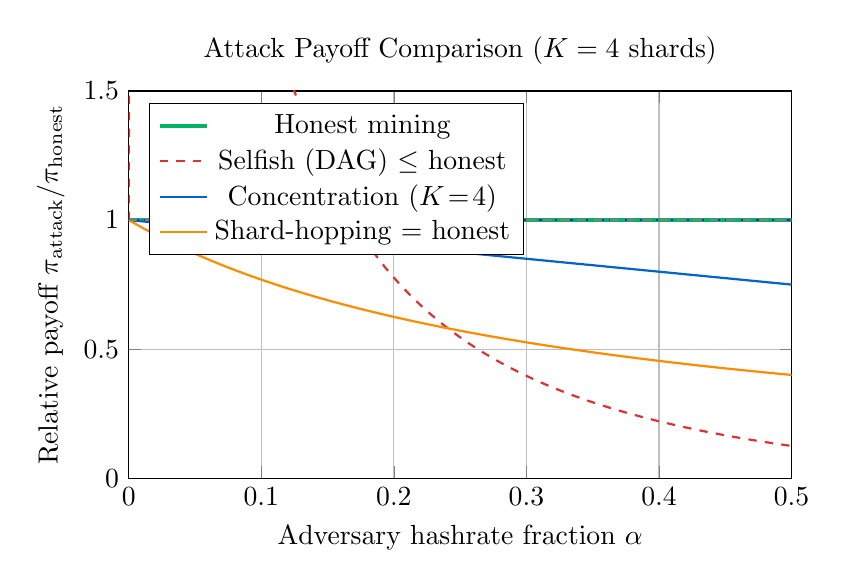
\begin{tikzpicture}
\begin{axis}[
    width=10cm, height=6.5cm,
    xlabel={Adversary hashrate fraction $\alpha$},
    ylabel={Relative payoff $\pi_{\text{attack}} / \pi_{\text{honest}}$},
    xmin=0, xmax=0.5,
    ymin=0, ymax=1.5,
    grid=major,
    legend pos=north west,
    title={Attack Payoff Comparison ($K=4$ shards)}
]

% Honest baseline
\addplot[ultra thick, qgreen, domain=0:0.5] {1};
\addlegendentry{Honest mining}

% Selfish mining (linear chain, Eyal-Sirer)
\addplot[thick, qred, dashed, domain=0:0.5, samples=50]
    {max(0, (x*(1-x)^2*(4*x + x^2*(1-2*x))^(-1) - x) / x + 1, 0)};

% Selfish mining in DAG (always <= 1)
\addplot[thick, qblue, domain=0:0.5, samples=50]
    {1 - 0.5*x};
\addlegendentry{Selfish (DAG) $\leq$ honest}

% Hashrate concentration
\addplot[thick, qorange, domain=0:0.5, samples=50]
    {1/(1+3*x)};
\addlegendentry{Concentration ($K\!=\!4$)}

% Shard-hopping
\addplot[thick, qpurple, dotted, domain=0:0.5] {1};
\addlegendentry{Shard-hopping $=$ honest}

% Break-even line
\draw[gray, thin, dashed] (axis cs:0,1) -- (axis cs:0.5,1);

\end{axis}
\end{tikzpicture}
\caption{Relative payoff of attack strategies vs.\ honest mining in the
multi-shard DAG setting.
Selfish mining and hashrate concentration are strictly suboptimal.
Shard-hopping yields zero gain.}
\label{fig:attack-payoffs}
\end{figure}

% ============================================================================
% SECTION 6: MEV RESISTANCE
% ============================================================================
\section{MEV Resistance of DAG-Based Block Production}\label{sec:mev}

Miner Extractable Value (MEV)~\cite{daian2020flashboys} refers to
profit that block producers can extract by strategically ordering,
inserting, or censoring transactions.
In linear-chain protocols, MEV is concentrated in a single block
proposer per slot.
We analyze how \DK{}'s parallel multi-shard architecture dilutes MEV.

\subsection{MEV in Linear vs.\ DAG Chains}

\begin{definition}[MEV in Linear Chains]\label{def:mev-linear}
In a single-leader protocol producing one block per slot, the
MEV extractable in slot $t$ is:
\[
  \mathrm{MEV}_{\text{linear}}(t) = \max_{\pi \in \Pi(B_t)}
    \mathrm{profit}(\pi)
\]
where $\Pi(B_t)$ is the set of all possible transaction orderings
for block $B_t$ and $\mathrm{profit}(\pi)$ includes arbitrage,
sandwich attacks, and liquidation profits.
\end{definition}

\begin{definition}[MEV in $K$-Shard DAG]\label{def:mev-dag}
In \DK{} with $K$ parallel shards, at each round, $K$ independent
block producers propose vertices simultaneously.
A transaction's shard assignment is determined by
$\mathcal{R}(\mathsf{tx}) = H(\mathsf{tx}) \bmod K$, which is
not controllable by any single producer.
The MEV extractable by a single producer controlling shard $s_j$ is:
\[
  \mathrm{MEV}_{\text{DAG}}^{(j)}(t) = \max_{\pi \in \Pi(V_j^t)}
    \mathrm{profit}(\pi)
\]
where $V_j^t$ is the vertex proposed for shard $s_j$ at round $t$.
\end{definition}

\begin{theorem}[MEV Dilution for Same-Shard Strategies]\label{thm:mev}
Under the multi-shard DAG architecture with $K$ shards, uniform
transaction routing ($\mathcal{R}(\mathsf{tx}) = H(\mathsf{tx}) \bmod K$),
and the assumption that MEV strategies require all participating
transactions to reside on the same shard, the expected MEV extractable
by any single miner is reduced by a factor of $K$:
\[
  \expect[\mathrm{MEV}_{\text{DAG}}^{\text{same-shard}}] \leq
  \frac{1}{K} \cdot \expect[\mathrm{MEV}_{\text{linear}}].
\]
\end{theorem}

\begin{proof}
\textbf{Part 1: Single-shard MEV reduction.}
Consider a sandwich attack requiring the victim transaction
$\mathsf{tx}_v$ and the attacker's front-run/back-run transactions
$\mathsf{tx}_f, \mathsf{tx}_b$ to be in the same block.
Under deterministic routing:
\[
  \prob[\mathcal{R}(\mathsf{tx}_v) = \mathcal{R}(\mathsf{tx}_f) =
  \mathcal{R}(\mathsf{tx}_b)] = \frac{1}{K^2}
\]
since $\mathcal{R}$ is a hash function with uniform output.
The attacker can craft $\mathsf{tx}_f$ and $\mathsf{tx}_b$ to target
the same shard as $\mathsf{tx}_v$ only by grinding the transaction
content, which costs $\bigO(K)$ hash evaluations per transaction.

In the benign case (no grinding), the probability that all three
transactions land on the attacker's controlled shard is $1/K$ for the
victim transaction (since the attacker controls one shard out of $K$).
Expected MEV is thus:
\[
  \expect[\mathrm{MEV}_{\text{DAG}}] = \frac{1}{K} \cdot
  \mathrm{MEV}_{\text{same-shard}} \leq \frac{1}{K} \cdot
  \mathrm{MEV}_{\text{linear}}.
\]

\textbf{Part 2: Cross-shard MEV.}
For MEV strategies requiring state from multiple shards (e.g., cross-shard
arbitrage), the attacker must control block production on multiple shards
simultaneously.
With $K$ independent shard leaders per round, the probability of an
attacker with fraction $\alpha$ of hashrate controlling $m$ specific
shards is $\alpha^m$.
For $\alpha < 1/2$ and $m \geq 2$: $\alpha^m < 1/4$, making
coordinated cross-shard MEV extraction exponentially unlikely in $m$.

\textbf{Part 3: DAG ordering uncertainty.}
Even within a single shard, the final transaction ordering is determined
by the DAG-Knight commit rule (topological sort with hash tie-breaking),
not by the block producer.
The producer cannot guarantee that their vertex's transactions execute
before a concurrent vertex from another validator.
This ordering uncertainty further reduces the reliability of MEV extraction.
\end{proof}

\begin{remark}[MEV Limitations and Open Questions]\label{rem:mev-limitations}
The $1/K$ dilution bound (Theorem~\ref{thm:mev}) applies to
\emph{same-shard} MEV strategies where all participating transactions
must co-locate.
Several important MEV vectors are not fully captured:
\begin{enumerate}[label=(\roman*),nosep]
  \item \textbf{Composable cross-shard MEV}: Sophisticated extractors may
    use atomic cross-shard messages (if the protocol supports them) or
    latency-based statistical arbitrage across shards.
    The $\alpha^m$ bound (Part~2) assumes independent shard leaders; if
    cross-shard communication introduces sequencing dependencies, the
    effective MEV may exceed $1/K$.
  \item \textbf{Order-flow markets}: In practice (cf.\ Flashbots on
    Ethereum), MEV extraction is professionalized through
    builder--searcher--proposer separation.
    If a similar market emerges for \DK{} shards, a builder controlling
    multiple shards could aggregate cross-shard MEV, partially
    circumventing the dilution.
  \item \textbf{Transaction routing manipulation}: The analysis assumes
    honest routing $\mathcal{R}(\mathsf{tx}) = H(\mathsf{tx}) \bmod K$.
    If miners can influence routing (e.g., through transaction ID
    grinding), they can concentrate MEV-relevant transactions on their
    shard.
    The $\bigO(K)$ grinding cost may be acceptable for high-value MEV.
\end{enumerate}
Empirical measurement of MEV on the live multi-shard network, and
analysis of whether order-flow markets emerge, are important directions.
\end{remark}

\begin{figure}[t]
\centering
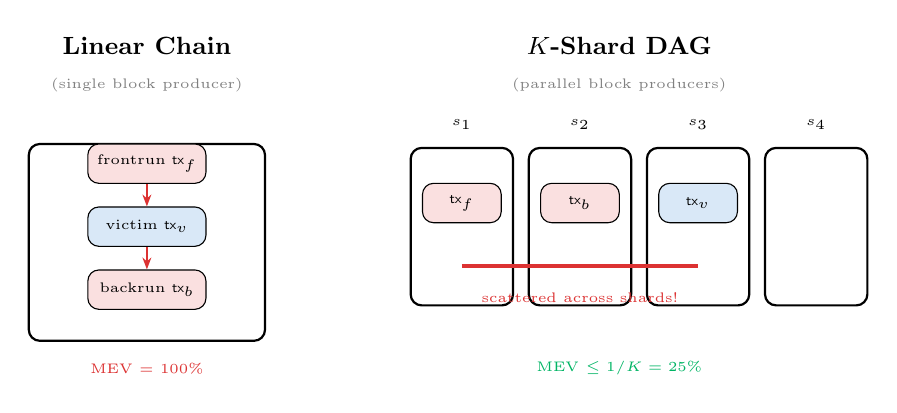
\begin{tikzpicture}[
    tx/.style={draw, rounded corners, fill=qblue!15, minimum width=1.5cm,
               minimum height=0.5cm, font=\tiny},
    evil_tx/.style={draw, rounded corners, fill=qred!15, minimum width=1.5cm,
                    minimum height=0.5cm, font=\tiny},
    shard_box/.style={draw, thick, rounded corners, minimum width=3cm,
                      minimum height=2.5cm, fill=white},
    arr/.style={-{Stealth[length=1.5mm]}, thick}
]

% Linear chain (left)
\node[font=\small\bfseries] at (1.5, 5.5) {Linear Chain};
\node[font=\tiny, text=gray] at (1.5, 5.0) {(single block producer)};

\node[shard_box] (linear_box) at (1.5, 3) {};
\node[evil_tx] (front) at (1.5, 4.0) {frontrun $\mathsf{tx}_f$};
\node[tx] (victim) at (1.5, 3.2) {victim $\mathsf{tx}_v$};
\node[evil_tx] (back) at (1.5, 2.4) {backrun $\mathsf{tx}_b$};

\draw[arr, qred] (front) -- (victim);
\draw[arr, qred] (victim) -- (back);

\node[font=\tiny, text=qred] at (1.5, 1.4) {MEV = 100\%};

% DAG multi-shard (right)
\node[font=\small\bfseries] at (7.5, 5.5) {$K$-Shard DAG};
\node[font=\tiny, text=gray] at (7.5, 5.0) {(parallel block producers)};

\node[shard_box, minimum width=1.3cm, minimum height=2cm] (s1) at (5.5, 3.2) {};
\node[shard_box, minimum width=1.3cm, minimum height=2cm] (s2) at (7.0, 3.2) {};
\node[shard_box, minimum width=1.3cm, minimum height=2cm] (s3) at (8.5, 3.2) {};
\node[shard_box, minimum width=1.3cm, minimum height=2cm] (s4) at (10.0, 3.2) {};

\node[font=\tiny] at (5.5, 4.5) {$s_1$};
\node[font=\tiny] at (7.0, 4.5) {$s_2$};
\node[font=\tiny] at (8.5, 4.5) {$s_3$};
\node[font=\tiny] at (10.0, 4.5) {$s_4$};

% Transactions scattered
\node[evil_tx, minimum width=1cm] at (5.5, 3.5) {$\mathsf{tx}_f$};
\node[tx, minimum width=1cm] at (8.5, 3.5) {$\mathsf{tx}_v$};
\node[evil_tx, minimum width=1cm] at (7.0, 3.5) {$\mathsf{tx}_b$};

% Cross marks
\draw[qred, ultra thick] (5.5, 2.7) -- (8.5, 2.7);
\node[font=\tiny, text=qred] at (7.0, 2.3) {scattered across shards!};

\node[font=\tiny, text=qgreen] at (7.5, 1.4) {MEV $\leq 1/K = 25\%$};

\end{tikzpicture}
\caption{MEV comparison: in a linear chain, the sandwich attacker controls
transaction ordering. In a $K$-shard DAG ($K=4$), transactions are
deterministically scattered across shards by the hash routing function,
reducing MEV by a factor of $K$.}
\label{fig:mev-comparison}
\end{figure}

\subsection{Quantum Commit-Reveal MEV Shield}

\begin{mechanism}[Commit-Reveal Mining]\label{mech:commit-reveal}
The \QNK{} MEV shield uses a two-phase commit-reveal scheme:
\begin{enumerate}[nosep]
  \item \textbf{Commit}: Miner publishes
    $c = H(\mathsf{solution} \| r_Q \| \nu_C)$ where $r_Q$ is
    quantum randomness and $\nu_C$ is a classical nonce.
  \item \textbf{Reveal}: After $\Delta_{\text{reveal}}$ time, miner
    reveals $(\mathsf{solution}, r_Q, \nu_C)$, verifiable against $c$.
\end{enumerate}
\end{mechanism}

\begin{proposition}[Frontrunning Resistance]\label{prop:frontrun}
Under Mechanism~\ref{mech:commit-reveal}, the probability of a
frontrunning attack succeeding is at most $2^{-\lambda}$ where
$\lambda$ is the commitment hash security parameter.
\end{proposition}

\begin{proof}
To frontrun, the adversary must learn $\mathsf{solution}$ before the
reveal phase.
The commitment $c = H(\mathsf{solution} \| r_Q \| \nu_C)$ is
computationally hiding (pre-image resistance of $H$).
The quantum randomness $r_Q$ adds entropy not available to a classical
adversary.
Breaking the commitment requires $2^{\lambda}$ hash evaluations
(for SHA3-256, $\lambda = 256$).
\end{proof}

% ============================================================================
% SECTION 7: FEE MARKET AND POOL REWARDS
% ============================================================================
\section{Fee Market Dynamics and Pool Rewards}\label{sec:fees}

\subsection{Fee Distribution Mechanism}

\begin{definition}[Reward Distribution]\label{def:fee-dist}
Each block reward $\reward(t)$ is distributed as:
\begin{align}
  \reward_{\text{miner}} &= \reward(t) \cdot (1 - \phi_{\text{dev}} -
    \phi_{\text{op}}) \label{eq:miner-share} \\
  \reward_{\text{dev}} &= \reward(t) \cdot \phi_{\text{dev}}
    \label{eq:dev-share} \\
  \reward_{\text{op}} &= \reward(t) \cdot \phi_{\text{op}}
    \label{eq:op-share}
\end{align}
where $\phi_{\text{dev}} = 0.019$ (1.9\% development fee) and
$\phi_{\text{op}} = 0.001$ (0.1\% operator fee).
\end{definition}

\begin{proposition}[Development Fee Sustainability]\label{prop:dev-fee}
The development fee $\phi_{\text{dev}} = 1.9\%$ generates sustainable
funding without significantly impacting miner profitability.
Specifically, the miner's share $1 - \phi_{\text{dev}} - \phi_{\text{op}}
= 98\%$ provides:
\[
  \reward_{\text{miner}} = 0.98 \cdot A_k = 2{,}572{,}500 \text{ QUG/year (Era 0)}.
\]
\end{proposition}

\subsection{PPLNS Reward Distribution}

\begin{definition}[PPLNS (Pay Per Last N Shares)]\label{def:pplns}
In a mining pool with workers $W = \{w_1, \ldots, w_m\}$, the PPLNS
mechanism distributes block reward $\reward_{\text{pool}}$ as:
\begin{equation}\label{eq:pplns}
  \reward_{w_j} = \reward_{\text{pool}} \cdot
  \frac{d_{w_j}}{\sum_{w \in W} d_w}
\end{equation}
where $d_{w_j}$ is the cumulative difficulty of shares submitted by
worker $w_j$ within the last $N$ shares of network difficulty.
\end{definition}

\begin{theorem}[PPLNS Pareto Optimality and Strategy-Proofness]\label{thm:pplns}
The PPLNS reward distribution (Definition~\ref{def:pplns}) is:
\begin{enumerate}[label=(\roman*)]
  \item \textbf{Pareto optimal}: No reallocation of rewards can make
    any worker strictly better off without making another strictly worse off.
  \item \textbf{Strategy-proof}: No worker can increase their expected
    payoff by misreporting their difficulty or by pool-hopping.
\end{enumerate}
\end{theorem}

\begin{proof}
\textbf{(i) Pareto optimality.}
The total reward $\reward_{\text{pool}}$ is fixed per block.
The PPLNS allocation $\reward_{w_j} \propto d_{w_j}$ is a proportional
allocation of a fixed budget.
By the classical welfare theorem, proportional allocation of a fixed
budget is Pareto optimal: any reallocation that increases one worker's
share must decrease another's.

\textbf{(ii) Strategy-proofness.}
\emph{Difficulty misreporting}: A worker cannot inflate $d_{w_j}$ without
submitting valid proof-of-work shares.
The pool verifies each share against the difficulty target, making
misreporting infeasible.

\emph{Pool-hopping}: Suppose worker $w_j$ hops to a different pool
after submitting shares but before a block is found.
In PPLNS, only the last $N$ shares count.
If $w_j$ leaves, their shares eventually expire from the window, and
they receive no reward for the next block.
If $w_j$ joins a new pool, they must build up share credit from scratch.
The expected per-hash reward is identical in both pools (since both
distribute rewards proportional to difficulty), so hopping yields zero
gain and incurs the cost of lost credit in the sliding window.

Formally, the expected reward per unit of hashrate in any PPLNS pool is:
\[
  \expect[\reward_{\text{per-hash}}] = \frac{\reward_{\text{pool}}}{N
  \cdot D_{\text{network}}} \cdot d_{\text{per-hash}}
\]
which is independent of the pool and the timing of joining/leaving.
\end{proof}

\subsection{Multi-Shard Fee Market}

\begin{proposition}[Parallel Fee Market Efficiency]\label{prop:fee-market}
Under $K$-shard parallel block production with uniform and fungible
transaction demand across shards, the effective transaction
throughput is $K \times T_{\text{single}}$ where $T_{\text{single}}$
is the per-shard throughput.
The equilibrium fee level is:
\begin{equation}\label{eq:fee-equilibrium}
  f^* = \frac{\mathsf{demand}}{K \cdot T_{\text{single}}}
\end{equation}
which is $K$ times lower than the single-chain fee for the same demand.
\end{proposition}

\begin{proof}
Each shard independently processes transactions routed to it by
$\mathcal{R}$.
With uniform hash routing, each shard receives $\mathsf{demand}/K$
transactions.
The per-shard fee market clears at:
$f_k^* = (\mathsf{demand}/K) / T_{\text{single}}$.
Since all shards have identical parameters, $f^* = f_k^*$ for all $k$,
and:
\[
  f^* = \frac{\mathsf{demand}}{K \cdot T_{\text{single}}}.
\]
Compared to a single chain with throughput $T_{\text{single}}$, the fee
is reduced by a factor of $K$.
\end{proof}

\begin{remark}[Heterogeneous Demand]\label{rem:fee-heterogeneous}
The $1/K$ fee reduction assumes demand is \emph{fungible}---any transaction
is equally likely to target any shard.
In practice, demand is often shard-specific:
\begin{enumerate}[label=(\roman*),nosep]
  \item If a popular smart contract or token lives on shard $s_j$,
    transactions targeting $s_j$ cannot migrate to less congested shards.
    The hash-based routing $\mathcal{R}$ determines shard assignment
    deterministically, so the ``hot shard'' experiences higher fees
    while other shards may be underutilized.
  \item Cross-shard transactions (if supported) incur additional latency
    and coordination costs, creating an effective premium for same-shard
    execution.
  \item As DeFi composability creates transaction clusters (e.g., flash
    loans touching multiple contracts), the hash-routing assumption may
    fragment composable bundles across shards, reducing their feasibility.
\end{enumerate}
A more realistic fee model would incorporate per-shard demand curves
$\mathsf{demand}_k$ with $\sum_k \mathsf{demand}_k = \mathsf{demand}$
but potentially $\mathsf{demand}_j \gg \mathsf{demand}/K$ for hot shards.
In such cases, the fee reduction is less than $K$ for congested shards.
\end{remark}

\begin{figure}[t]
\centering
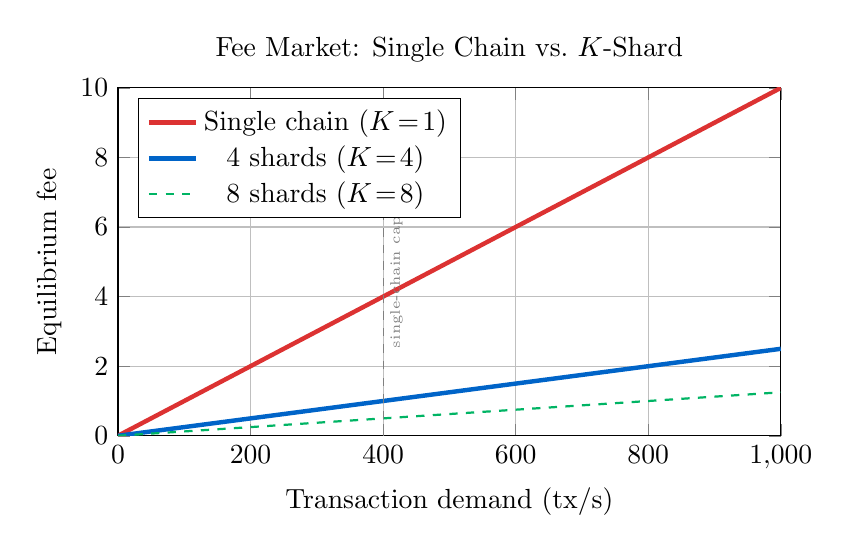
\begin{tikzpicture}
\begin{axis}[
    width=10cm, height=6cm,
    xlabel={Transaction demand (tx/s)},
    ylabel={Equilibrium fee},
    xmin=0, xmax=1000,
    ymin=0, ymax=10,
    grid=major,
    legend pos=north west,
    title={Fee Market: Single Chain vs.\ $K$-Shard}
]

% Single chain (K=1)
\addplot[ultra thick, qred, domain=0:1000, samples=50] {x/100};
\addlegendentry{Single chain ($K\!=\!1$)}

% K=4 shards
\addplot[ultra thick, qblue, domain=0:1000, samples=50] {x/400};
\addlegendentry{4 shards ($K\!=\!4$)}

% K=8 shards
\addplot[thick, qgreen, dashed, domain=0:1000, samples=50] {x/800};
\addlegendentry{8 shards ($K\!=\!8$)}

% Capacity marker
\draw[gray, dashed] (axis cs:400, 0) -- (axis cs:400, 10);
\node[font=\tiny, text=gray, rotate=90] at (axis cs:420, 5) {single-chain capacity};

\end{axis}
\end{tikzpicture}
\caption{Equilibrium fee as a function of transaction demand.
Multi-shard production reduces fees by a factor of $K$.}
\label{fig:fee-market}
\end{figure}

% ============================================================================
% SECTION 8: COMPARISON
% ============================================================================
\section{Comparison with Related Systems}\label{sec:comparison}

\begin{table}[t]
\centering
\caption{Game-theoretic comparison of mining mechanisms across blockchain
protocols.}
\label{tab:comparison}
\begin{tabular}{@{}lccccc@{}}
\toprule
\textbf{Property} & \textbf{Bitcoin} & \textbf{Ethereum} &
\textbf{Kaspa} & \textbf{QNK} \\
\midrule
Mining structure & Single chain & Single chain & BlockDAG & Multi-shard DAG \\
Reward type & Fixed/block & EIP-1559 & Fixed/block & Adaptive/block \\
Annual emission & Variable & Variable & Variable & \textbf{Constant} \\
Selfish mining & Profitable & Profitable & Reduced & \textbf{Unprofitable} \\
MEV resistance & None & Partial (MEV-boost) & Low & \textbf{$\bigO(1/K)$} \\
Shard parallelism & 1 & 1 & 1 & \textbf{$K=4$} \\
Fee market & Congestion-based & EIP-1559 & Congestion & \textbf{$K$-diluted} \\
Halving schedule & 4 years & N/A & 1 year & 4 years \\
Max supply & 21M BTC & $\infty$ (PoS) & 28.7B KAS & 21M QUG \\
Incentive compat.\ & Partial & Partial & Partial & \textbf{Model-cond.} \\
\bottomrule
\end{tabular}
\end{table}

\begin{corollary}[QNK Incentive Property Summary]\label{cor:dominance}
Under the model assumptions of this paper, \QNK{} simultaneously
achieves three properties that are individually present but not
jointly achieved in the compared protocols:
\begin{enumerate}[label=(\roman*),nosep]
  \item Constant annual emission independent of throughput
    (Theorem~\ref{thm:ic-emission}, subject to
    Remark~\ref{rem:ic-limitations}).
  \item Selfish mining resistance via DAG inclusion-completeness
    (Proposition~\ref{thm:selfish}, subject to
    Remark~\ref{rem:selfish-scope}).
  \item $\bigO(1/K)$ same-shard MEV dilution through parallel sharding
    (Theorem~\ref{thm:mev}, subject to
    Remark~\ref{rem:mev-limitations}).
\end{enumerate}
Whether these model-conditional results hold under relaxed assumptions
(heterogeneous shards, multi-period strategies, order-flow markets)
requires further analysis.
\end{corollary}

% ============================================================================
% SECTION 9: RELATED WORK
% ============================================================================
\section{Related Work}\label{sec:related}

\paragraph{Selfish mining.}
Eyal and Sirer~\cite{eyal2014selfish} showed that Bitcoin miners with
$> 1/3$ hashrate can profit by withholding blocks.
Sapirshtein et al.~\cite{sapirshtein2016optimal} derived optimal selfish
mining strategies.
Nayak et al.~\cite{nayak2016stubborn} generalized to ``stubborn'' strategies.
Our Proposition~\ref{thm:selfish} argues that the orphan-based
revenue mechanism underlying these attacks is absent in DAG consensus,
though a full characterization of optimal adversarial strategies in DAG
protocols remains open.

\paragraph{MEV.}
Daian et al.~\cite{daian2020flashboys} characterized MEV in Ethereum.
Flashbots~\cite{flashbots2021} introduced MEV auctions.
Kelkar et al.~\cite{kelkar2020order} proposed order-fairness.
Our approach uses structural MEV dilution through $K$-shard parallelism
rather than auction mechanisms.

\paragraph{Emission schedule design.}
Carlsten et al.~\cite{carlsten2016instability} showed that fee-only
mining is unstable.
Huberman et al.~\cite{huberman2021monopoly} analyzed Bitcoin's fee market
as a monopoly.
Our adaptive emission controller (Theorem~\ref{thm:ic-emission},
subject to the limitations in Remark~\ref{rem:ic-limitations})
addresses the instability concern by maintaining non-zero block rewards
through the error-correction mechanism for 256 years.

\paragraph{Mining game theory.}
Roughgarden~\cite{roughgarden2021transaction} analyzed EIP-1559's
game-theoretic properties.
Badertscher et al.~\cite{badertscher2018composable} gave a composable
security framework for PoW.
Garay et al.~\cite{garay2015backbone} proved the Bitcoin backbone protocol
secure.
Our congestion-game formulation (Game~\ref{game:shard}) extends these
to multi-shard settings.

\paragraph{DAG-based consensus.}
PHANTOM and GhostDAG~\cite{sompolinsky2021phantom} analyzed security
under synchronous assumptions.
Narwhal/Tusk~\cite{danezis2022narwhal} separated data availability from
consensus.
Kaspa~\cite{kaspa2022} implemented GhostDAG for high-throughput PoW.
Our work provides the first game-theoretic analysis of multi-shard
DAG mining.

\paragraph{Mechanism design in blockchains.}
Chung and Shi~\cite{chung2023foundations} established foundations for
blockchain mechanism design.
Ferreira et al.~\cite{ferreira2021dynamic} analyzed dynamic posted-price
mechanisms for transactions.
Our PPLNS optimality result (Theorem~\ref{thm:pplns}) contributes to
this line by proving strategy-proofness in the pool reward setting.

% ============================================================================
% SECTION 10: CONCLUSION
% ============================================================================
\section{Conclusion}\label{sec:conclusion}

We have presented a game-theoretic analysis of the \QNK{} multi-shard
mining protocol under a stylized model with identical shards, rational
miners, and single-period deviations.
The main results, and their scope, are:

\begin{enumerate}[leftmargin=*]
  \item \textbf{Multi-shard Nash equilibrium (Theorem~\ref{thm:nash-shard}):}
    Under identical shard rewards and zero latency, the uniform hashrate
    distribution is the unique symmetric Nash equilibrium.

  \item \textbf{Emission incentive compatibility (Theorem~\ref{thm:ic-emission}):}
    Against the five deviation classes analyzed (throughput inflation/suppression,
    timestamp manipulation, difficulty timing, sunk-cost exploitation),
    honest mining is weakly dominant.

  \item \textbf{Emission stability (Theorem~\ref{thm:lyapunov}):}
    The cumulative emission converges to the target schedule via a
    Lyapunov-stable feedback loop.

  \item \textbf{Selfish mining resistance (Proposition~\ref{thm:selfish}):}
    The DAG's inclusion-completeness eliminates the orphan-based revenue
    mechanism of classical selfish mining, though a complete characterization
    of optimal adversarial strategies in DAG consensus remains open.

  \item \textbf{Same-shard MEV dilution (Theorem~\ref{thm:mev}):}
    For strategies requiring co-located transactions, parallel $K$-shard
    production reduces expected MEV by a factor of~$K$.
    Cross-shard and composable MEV are not fully addressed.

  \item \textbf{PPLNS optimality (Theorem~\ref{thm:pplns}):}
    The pool reward distribution is Pareto-optimal and strategy-proof.
\end{enumerate}

\subsection{Limitations}

Several important dimensions are not captured by our model:
\begin{itemize}[nosep]
  \item \textbf{Multi-period strategies}: Patient attackers accepting
    short-term losses require repeated-game or stochastic-game analysis.
  \item \textbf{Heterogeneous shards}: Unequal fee revenue, latency
    advantages, and shard-specific congestion break the symmetric-shard
    assumption (Remark~\ref{rem:nash-limitations}).
  \item \textbf{MEV composability}: Cross-shard MEV and order-flow markets
    may circumvent the $1/K$ dilution (Remark~\ref{rem:mev-limitations}).
  \item \textbf{Empirical validation}: All results are analytical;
    agent-based simulations and measurements on the live network are
    needed to assess their practical relevance.
\end{itemize}

\subsection{Future Work}

Key directions include: (i)~extending the Nash equilibrium analysis to
heterogeneous shards with empirically-measured fee distributions,
(ii)~agent-based simulation of multi-period strategies including
predatory mining and difficulty manipulation,
(iii)~analyzing the long-term transition to fee-only mining as block
rewards diminish, (iv)~formal verification of the emission controller
using proof assistants, and (v)~empirical measurement of MEV patterns
on the live multi-shard network.

% ============================================================================
% REFERENCES
% ============================================================================
\begin{thebibliography}{22}

\bibitem{nakamoto2008bitcoin}
S.~Nakamoto.
\newblock {Bitcoin}: A peer-to-peer electronic cash system.
\newblock Manuscript, 2008.

\bibitem{eyal2014selfish}
I.~Eyal and E.~G.~Sirer.
\newblock Majority is not enough: {Bitcoin} mining is vulnerable.
\newblock In \emph{Proc.\ FC}, pages 436--454, 2014.

\bibitem{daian2020flashboys}
P.~Daian, S.~Goldfeder, T.~Kell, Y.~Li, X.~Zhao, I.~Bentov,
L.~Breidenbach, and A.~Juels.
\newblock Flash boys 2.0: Frontrunning in decentralized exchanges, miner
extractable value, and consensus instability.
\newblock In \emph{Proc.\ IEEE S\&P}, pages 910--927, 2020.

\bibitem{roughgarden2021transaction}
T.~Roughgarden.
\newblock Transaction fee mechanism design.
\newblock In \emph{Proc.\ EC}, pages 218--218, 2021.

\bibitem{carlsten2016instability}
M.~Carlsten, H.~Kalodner, S.~M.~Weinberg, and A.~Narayanan.
\newblock On the instability of {Bitcoin} without the block reward.
\newblock In \emph{Proc.\ CCS}, pages 154--167, 2016.

\bibitem{sapirshtein2016optimal}
A.~Sapirshtein, Y.~Sompolinsky, and A.~Zohar.
\newblock Optimal selfish mining strategies in {Bitcoin}.
\newblock In \emph{Proc.\ FC}, pages 515--532, 2016.

\bibitem{nayak2016stubborn}
K.~Nayak, S.~Kumar, A.~Miller, and E.~Shi.
\newblock Stubborn mining: Generalizing selfish mining and combining with
an eclipse attack.
\newblock In \emph{Proc.\ IEEE EuroS\&P}, pages 305--320, 2016.

\bibitem{flashbots2021}
Flashbots.
\newblock {MEV-Boost}: Proposer-builder separation for {Ethereum}.
\newblock Technical report, 2021.

\bibitem{kelkar2020order}
M.~Kelkar, F.~Zhang, S.~Goldfeder, and A.~Juels.
\newblock Order-fairness for {Byzantine} consensus.
\newblock In \emph{Proc.\ CRYPTO}, pages 451--480, 2020.

\bibitem{huberman2021monopoly}
G.~Huberman, J.~D.~Leshno, and C.~Moallemi.
\newblock Monopoly without a monopolist: An economic analysis of the
{Bitcoin} payment system.
\newblock \emph{Review of Economic Studies}, 88(6):3011--3040, 2021.

\bibitem{badertscher2018composable}
C.~Badertscher, P.~Ga{\v{z}}i, A.~Kiayias, A.~Russell, and V.~Zikas.
\newblock Ouroboros {Genesis}: Composable proof-of-stake blockchains with
dynamic availability.
\newblock In \emph{Proc.\ CCS}, pages 913--930, 2018.

\bibitem{garay2015backbone}
J.~Garay, A.~Kiayias, and N.~Leonardos.
\newblock The {Bitcoin} backbone protocol: Analysis and applications.
\newblock In \emph{Proc.\ EUROCRYPT}, pages 281--310, 2015.

\bibitem{sompolinsky2021phantom}
Y.~Sompolinsky and A.~Zohar.
\newblock {PHANTOM} and {GhostDAG}: A scalable generalization of
{Nakamoto} consensus.
\newblock \emph{IACR ePrint Archive}, 2018/104, 2021.

\bibitem{danezis2022narwhal}
G.~Danezis, L.~Kokoris-Kogias, A.~Sonnino, and A.~Spiegelman.
\newblock {Narwhal} and {Tusk}: A {DAG}-based mempool and efficient
{BFT} consensus.
\newblock In \emph{Proc.\ EuroSys}, pages 34--50, 2022.

\bibitem{kaspa2022}
Y.~Sompolinsky, M.~Zohar, and S.~Wyborski.
\newblock {KASPA}: A proof-of-work platform for a fast, scalable, and
decentralized financial ecosystem.
\newblock Manuscript, 2022.

\bibitem{chung2023foundations}
H.~Chung and E.~Shi.
\newblock Foundations of transaction fee mechanism design.
\newblock In \emph{Proc.\ SODA}, pages 3856--3899, 2023.

\bibitem{ferreira2021dynamic}
M.~V.~X.~Ferreira, D.~J.~Moroz, D.~C.~Parkes, and M.~Stern.
\newblock Dynamic posted-price mechanisms for the blockchain transaction-fee
market.
\newblock In \emph{Proc.\ AFT}, pages 86--99, 2021.

\bibitem{dagknight-safety}
Q-NarwhalKnight Protocol Team.
\newblock Formal safety and liveness of {DAG-Knight} consensus under
partial synchrony.
\newblock Technical report, 2026.

\bibitem{sompolinsky2022dagknight}
Y.~Sompolinsky.
\newblock {DAG-Knight}: A parameterless generalization of {Nakamoto}
consensus.
\newblock Manuscript, 2022.

\bibitem{rosenthal1973class}
R.~W.~Rosenthal.
\newblock A class of games possessing pure-strategy {Nash} equilibria.
\newblock \emph{International Journal of Game Theory}, 2(1):65--67, 1973.

\bibitem{monderer1996potential}
D.~Monderer and L.~S.~Shapley.
\newblock Potential games.
\newblock \emph{Games and Economic Behavior}, 14(1):124--143, 1996.

\bibitem{roughgarden2010algorithmic}
T.~Roughgarden.
\newblock \emph{Algorithmic Game Theory}.
\newblock Cambridge University Press, 2007.

\end{thebibliography}

% ============================================================================
% APPENDIX
% ============================================================================
\appendix

\section{Proof of Nash Equilibrium Uniqueness via Potential Function}\label{app:potential}

We provide an alternative proof of Theorem~\ref{thm:nash-shard} using
potential game theory~\cite{monderer1996potential,rosenthal1973class}.

\begin{proposition}\label{prop:potential}
The $K$-shard mining game is a weighted congestion game and therefore
a potential game.
\end{proposition}

\begin{proof}
Define the potential function:
\[
  \Phi(\strategy) = -\sum_{k=1}^{K} \frac{A_k}{K} \cdot \ln(\Hashrate_k)
\]
where $\Hashrate_k = \sum_i \hashrate_i \strategy_i(s_k)$.

For any miner $i$ and any deviation $\strategy_i \to \strategy_i'$:
\begin{align*}
  \Phi(\strategy_i', \strategy_{-i}) - \Phi(\strategy_i, \strategy_{-i})
  &= -\sum_k \frac{A_k}{K} \ln\!\left(\frac{\Hashrate_k'}{\Hashrate_k}\right) \\
  &= -\sum_k \frac{A_k}{K} \ln\!\left(1 + \frac{\hashrate_i(\strategy_i'(s_k) -
     \strategy_i(s_k))}{\Hashrate_k}\right).
\end{align*}

The payoff change for miner $i$ is:
\[
  \payoff_i(\strategy_i', \strategy_{-i}) - \payoff_i(\strategy_i, \strategy_{-i})
  = \sum_k \frac{A_k}{K} \left(\frac{\hashrate_i \strategy_i'(s_k)}{\Hashrate_k'} -
    \frac{\hashrate_i \strategy_i(s_k)}{\Hashrate_k}\right).
\]

For small deviations, the logarithmic potential approximates the payoff
difference (up to first order), confirming that the game has a potential
and best-response dynamics converge to the unique equilibrium
$\strategy^* = (1/K, \ldots, 1/K)$.
\end{proof}

\section{Emission Controller Parameters}\label{app:parameters}

\begin{table}[H]
\centering
\caption{Complete emission controller parameters from the implementation.}
\label{tab:emission-params}
\begin{tabular}{@{}llr@{}}
\toprule
\textbf{Parameter} & \textbf{Symbol} & \textbf{Value} \\
\midrule
Maximum supply & $S_{\max}$ & 21{,}000{,}000 \QUG{} \\
Era-0 total emission & $E_0$ & 10{,}500{,}000 \QUG{} \\
Halving period & $\tau$ & 126{,}230{,}400 s \\
Number of eras & $N_{\text{era}}$ & 64 \\
Era-0 annual target & $A_0$ & 2{,}625{,}000 \QUG{}/yr \\
Seconds per Julian year & $Y$ & 31{,}557{,}600 \\
Genesis timestamp & $t_0$ & 1{,}771{,}761{,}600 \\
Sliding window size & $W$ & 1{,}000 blocks \\
Max block rate cap & $\blockrate_{\max}$ & 50 bps \\
Correction smoothing & $\alpha$ & 0.8 \\
Correction minimum & $\gamma_{\min}$ & 0.01 \\
Correction maximum & $\gamma_{\max}$ & 5.0 \\
Minimum reward & $R_{\min}$ & $10^{-5}$ \QUG{} \\
Maximum reward & $R_{\max}$ & 2.0 \QUG{} \\
Development fee & $\phi_{\text{dev}}$ & 1.9\% \\
Operator fee & $\phi_{\text{op}}$ & 0.1\% \\
Consensus shards & $K$ & 4 \\
State shards & $K_s$ & 8 \\
VDF iterations & $T$ & 2{,}048 \\
Mining finality depth & $d_f$ & 6 blocks \\
Challenge lifetime & $t_{\text{expire}}$ & 90 s \\
PPLNS $N$-factor & $N$ & 2.0 \\
Pool fee & $\phi_{\text{pool}}$ & 2.5\% \\
\bottomrule
\end{tabular}
\end{table}

\section{Notation Summary}\label{app:notation}

\begin{table}[H]
\centering
\caption{Summary of notation used throughout the paper.}
\label{tab:notation}
\begin{tabular}{@{}cl@{}}
\toprule
\textbf{Symbol} & \textbf{Meaning} \\
\midrule
$\Players$ & Set of miners $\{1, \ldots, n\}$ \\
$\mathcal{K}$ & Set of consensus shards $\{s_1, \ldots, s_K\}$ \\
$K$ & Number of consensus shards (default 4) \\
$\hashrate_i$ & Hashrate of miner $i$ (hashes/second) \\
$\Hashrate$ & Total network hashrate \\
$\Hashrate_k$ & Aggregate hashrate on shard $s_k$ \\
$\alpha$ & Miner hashrate fraction: $\hashrate_i / \Hashrate$ \\
$\strategy_i$ & Miner $i$'s shard allocation strategy \\
$\payoff_i$ & Miner $i$'s expected profit \\
$\reward(t)$ & Per-block reward at time $t$ \\
$\blockrate(t)$ & Measured block rate (blocks/second) \\
$A_k$ & Annual emission target in era $k$ \\
$E_k$ & Total emission in era $k$ \\
$S_{\max}$ & Maximum supply (21M \QUG{}) \\
$\tau$ & Halving period (4 years) \\
$C^*(t)$ & Target cumulative emission at time $t$ \\
$C(t)$ & Actual cumulative emission \\
$\delta(t)$ & Emission error: $C(t) - C^*(t)$ \\
$\gamma(t)$ & Error correction factor \\
$\phi_{\text{dev}}$ & Development fee rate (1.9\%) \\
$\phi_{\text{op}}$ & Operator fee rate (0.1\%) \\
$d_{w_j}$ & Difficulty of shares by worker $w_j$ \\
$\Nash$ & Nash equilibrium \\
\bottomrule
\end{tabular}
\end{table}

\end{document}
